\section{Security and Privacy Analysis}
\label{sec:analysis}
We define three adversarial scenarios under the threat model in Section \ref{subsec:threatmodel}, develop a Dolev-Yao-style model \cite{BrowserID} to depict the SSO login flow,
 and formally prove the security and privacy guarantees provided by \usso\ using the conditions analyzed in the Dolev-Yao-style model.

\newc
\subsection{Adversarial Scenarios}

Based on our design goals (i.e., the desired security and privacy guarantees) and the potential adversaries discussed in Section \ref{subsec:threatmodel}, we consider three adversarial scenarios as below.

\noindent\textbf{Security.} Malicious users could collude with each other or with malicious RPs, attempting to (\emph{a}) impersonate an honest user to log into an honest RP or (\emph{b}) entice an honest user to log into an honest RP under a malicious user's account.

\noindent\textbf{Privacy against the IdP.}
The honest-but-curious IdP tries to infer the identities of the RPs that a user requests to access. %or link multiple logins to any RP initiated by a user.

\noindent\textbf{Privacy against RPs.}
Malicious RPs could collude with each other or with malicious users, attempting to link logins across these RPs that are initiated by a user.
\oldc

% \textcolor{blue}{Based on the threat model and assumptions proposed in Section \ref{sec:UPPRESSO},
%     different types of adversaries are considered in the analysis of security and privacy.
% First of all, in the proofs of security,
%     malicious RPs collude with malicious users,
%         attempting
%         to break any of the four security properties of SSO identity tokens for an honest user to visit an honest RP.
% Then, in the analysis of privacy against the IdP-based login tracing,
%    an honest-but-curious IdP is the only adversary.
% Finally,
%     in the privacy analysis against the RP-based identity linkage,
%     a number of malicious RPs collude, attempting to link an honest user's accounts across these RPs.}

% We first analyzed UPPRESSO %especially confidentiality and integrity,
%      based on a Dolev-Yao-style model \cite{SPRESSO}.
% % which has been used in the formal analysis of SSO protocols such as OAuth 2.0 \cite{FettKS16} and OIDC \cite{FettKS17}.
% The model abstracts the entities in a web system,
%     such as web servers and browsers,
%     as \emph{atomic processes}. %which communicate with each other through events. % such as HTTPS requests and responses.
% It defines \emph{script processes} to formulate client-side scripts.
% %The script is dependently invoked by the browser to process the server-defined logic.
%   %such as verifying $Certificate_{RP}$.
% %
% %postmessage events;
% %
% %atomic process <-> script process, communication.
% %
% %Other events change self-trigger.
% %
% UPPRESSO contains atomic processes including:
% an IdP process,
%     a finite set of web servers for honest RPs, a finite set of honest browsers, and a finite set of attacker processes.
% The processes communicate with each other through events such as HTTPS requests and responses.
% %We consider all RP and browser processes are honest,
% An RP or a browser controlled by adversaries is modeled as an attacker process.
% Within a browser,
%  an honest IdP script, an honest RP script, and also attacker scripts which are downloaded from attacker processes,
%   are invoked.
% %Although the scripts coexist in the same browser, they are strictly separated.
% Script processes communicate with each other through \verb+postMessage+,
%     modelled as transmitted-to-itself events of a browser process.
% %To clearly indicate the action of postMessage communication, we define it as the transmitting-to-itself event of the browser (which is not defined in SPRESSO).


% \textcolor{blue}{After formulating the system by this model,
%     we analyze the following data for the proofs in Sections \ref{analysis-security} and \ref{sec-:analysis},
%      when there are corresponding adversaries.
% We (\emph{a}) trace the lifecycle of an identity token for an honest user to visit an honest RP,
%         starting when it is generated and ending when accepted by the RP,
%     to ensure it is not leaked to adversaries,
% (\emph{b})
%     locate all places
%         where $PID_U$, $PID_{RP}$ and other parameters enclosed in the token are processed,
%      to ensure no adversary able to manipulate them,
% and (\emph{c})
%     locate the places where $PK$ is transmitted and used in the IdP script,
%         to ensure no adversary tampering with it.
% These conclusions are used to prove security of the UPPRESSO protocols.}
% %
% % to ensure it is not leaked to attackers or tampered with by any adversary without checking.
% \textcolor{blue}{In the meantime,
%         this model ensures that (\emph{a}) $t$ is unaccessible to the honest-but-curious IdP,
%  which is necessary to prevent the IdP-based login tracing,
%  and (\emph{b}) $u$ and $r$ are not leaked to RPs in the protocols,
%     necessary to prevent the RP-based identity linkage.}


%Next, we prove that \usso\ is secure in the first adversarial scenario in Section~\ref{analysis-security} and it can prevent privacy threats in the other two adversarial scenarios in Section~\ref{sec-:analysis}.


%The RP cannot derive $ID_U$ from either $PID_U$ or $Acct$ due to the elliptic curve discrete logarithm problem (ECDLP). Since $t$ is random in $\mathbb{Z}_n$ and unknown to the IdP, from the IdP's view, $PID_{RP}$ is indistinguishable from a random variable on $\mathbb{E}$. So, the IdP cannot learn anything about $ID_{RP}$ from $PID_{RP}$.
%Section \ref{sec:analysis} presents more detailed analyses.

\subsection{The Dolev-Yao-Style Model for \usso}
\label{dy-model}

We develop a Dolev-Yao style model \cite{BrowserID, SPRESSO, FettKS16, FettKS17} for \usso, referred to as the \dyu\ model, to formalize the login flow of \usso.
% Dolev-Yao style models abstract cryptographic concepts into an algebra of symbolic messages to discover structural flaws using simple formal logic. % which has been used in the formal analysis of SSO protocols such as OAuth 2.0 \cite{FettKS16} and OIDC \cite{FettKS17}.
The model abstracts the entities in a web system, such as web servers and browsers, as atomic processes, %which communicate with each other through events. % such as HTTPS requests and responses.
and defines script processes to formulate client-side scripts.
%The script is dependently invoked by the browser to process the server-defined logic.%such as verifying $Certificate_{RP}$. %postmessage events; %atomic process <-> script process, communication. %Other events change self-trigger.
The atomic processes of \usso\ include an IdP process, a finite set of web servers for honest RPs, a finite set of honest browsers, and a finite set of attacker processes that model malicious RPs and malicious users.
A browser may invoke an honest IdP script and multiple RP scripts that could be honest or malicious.
The processes communicate with each other through events such as HTTPS requests and responses,
%Although the scripts coexist in the same browser, they are strictly separated.
except that the script processes communicate with each other through \verb+postMessage+ which are modeled as transmitted-to-itself events of a browser process.
%To clearly indicate the action of postMessage communication, we define it as the transmitting-to-itself event of the browser (which is not defined in SPRESSO).

\newc
Applying the \dyu\ model, we trace the lifecycle of an identity token from its generation at the IdP to its acceptance at an RP, locate the places where $PID_U$, $PID_{RP}$, and other elements related to the identity token such as $t$ and $u$ are processed, and locate the places where $PK$ is transmitted and used in the IdP script.
We confirm the following conclusions in the \dyu\ model:
 (\emph{a}) an identity token binding pseudo-identities of honest entities, cannot be leaked to any malicious process;
 (\emph{b}) pseudo-identities and other elements in verified identity tokens cannot be manipulated by any malicious process;
    (\emph{c}) the IdP's public key set in the IdP script cannot be replaced or tampered with by any malicious process, within an honest browser;
 (\emph{d}) the IdP receives nothing about $t$ shared between two honest processes;
 (\emph{e}) $r$ is not leaked to any malicious process as it never leaves the IdP;
and (\emph{f}) the RPs cannot receive anything about $u$ shared between two honest processes.

%With the DYU model, we (\emph{a}) trace the lifecycle of an identity token from its generation at the IdP to its acceptance at an RP to prove that it cannot be leaked to adversaries; (\emph{b}) locate the places where $PID_U$, $PID_{RP}$, and other elements in the identity token are processed to prove that they cannot be manipulated by any adversary; and (\emph{c}) locate the places where $PK$ is transmitted and used in the IdP script to prove that it cannot be replaced by any adversary.


\subsection{Security}
\label{analysis-security}

%A secure SSO system allows a \emph{legitimate} user to login to an \emph{honest} RP with her account at this RP,
% by presenting \emph{identity tokens} issued by a \emph{trusted} IdP.

We prove that identity tokens in \usso\ and the enclosed pseudo-identities satisfy four properties, namely, \emph{RP designation}, \emph{user identification}, \emph{token confidentiality}, and \emph{token integrity}, which together ensure the security of \usso\ in the first adversarial scenario.
Let us consider an identity token $TK$ binding $PID_{RP}$ and $PID_U$, which is generated by the IdP upon a request from an authenticated user with $ID_U$.

%These conclusions are used to prove the security of the UPPRESSO protocols.
%We consider an arbitrary login in which an arbitrary RP with $ID_{RP}$ receives an integer $t$ and an identity token $TK$ issued by the IdP, binding a $PID_U$ and a $PID_{RP}$, from the RP script in a user browser. $TK$ is considered a valid identity token if the RP could verify its signature using the IdP's public key $PK$.

\vspace{2mm}
\noindent\textsc{\textbf{Theorem 1.} (RP Designation of $TK$)} { $PID_{RP}$ in $TK$ uniquely designates an RP with $ID_{RP}$, where $PID_{RP}= [t]ID_{RP}$, $t \in [1,n)$, $ID_{RP} = [r]G$, $r$ is a random number known only to the IdP, and $G$ is a generator on $\mathbb{E}$ of order $n$.}
%{\em Provided that $r$ is known only to the IdP, $PID_{RP}$ in the identity token uniquely designates the RP with $ID_{RP} = [r]G$.}}
%{\em If $TK$ is a valid identity token and $PID_{RP} = [t]ID_{RP}$ is satisfied, $PID_{RP}$ uniquely designates the RP that receives $TK$.}

\vspace{0.85mm}
\noindent\textsc{Proof.} In \usso, $PID_{RP}=[t]ID_{RP}$ is generated by a user based on the target RP's identity $ID_{RP}$ and a user-selected random number $t \in [1,n)$.
The target RP with $ID_{RP}$ receives $t$,
     and it will also calculate $PID_{RP}=[t]ID_{RP}$ to match $PID_{RP}$ extracted from a token received.
%It is computationally easy for any party who knows $ID_{RP}$ and $t$ to validate the $PID_{RP}$ in an identity token. A valid
Thus, $PID_{RP}$ always specifies an RP, i.e., %$PID_{RP}$ sent by a user in her identity-token request is calculated as $PID_{RP} = [t]ID_{RP}$, where $ID_{RP}$ is the target RP's identity and $t$ is a random number selected by the user and shared with this RP.
designates the target RP that knows $t$.

Next, according to Lemma 1, given $PID_{RP} = [t]ID_{RP}$, the probability that $PID_{RP}$ designates another RP with $ID_{RP'}$ is negligible. %This means that $PID_{RP}$ cannot be associated with any other RPs in the system.
Therefore, $PID_{RP}$ designates only the target RP with $ID_{RP}$ in the system.  \hfill $\square$

\vspace{2mm}
\noindent\textsc{\textbf{Lemma 1.}} { For any two RPs in a finite set of RPs, the probability of finding different numbers $t$ and $t' \in [1,n)$ that satisfy $[t]ID_{RP_j} = [t']ID_{RP_{j'}}$ is negligible, where $ID_{RP_j}=[r]G$, $ID_{RP_{j'}}=[r']G$, $r$ and $r'$ are different numbers unknown to the RPs, and $G$ is a generator on $\mathbb{E}$ of order $n$.}

%Based on the ECDLP we prove that, for adversaries, the probability of finding $t$ and $t'$ satisfying $[t]ID_{RP_j} = [t']ID_{RP_{j'}}$ is negligible, where $RP_j$ and $RP_{j'}$ are any two RPs in the finite set of RPs (i.e., $ID_{RP_j} = [r_j]G$ and $ID_{RP_{j'}} = [r_{j'}]G$, while $r_j$ and $r_{j'}$ are kept secret to the adversaries). This negligible probability means $PID_{RP_j} = [t]ID_{RP_j}$ designates \emph{only} the target RP with $ID_{RP_j}$.

\oldc
\vspace{0.85mm}
\noindent\textsc{Proof.}
Finding $t$ and $t'$ that satisfy $[t]ID_{RP_j} = [t']ID_{RP_{j'}}$, can be described as a $PID_{RP}$-collision game $\mathcal{G}_c$ between an adversary and a challenger: the adversary receives from the challenger a finite set of RP identities, i.e., $ID_{RP_1}$, ..., $ID_{RP_m}$, where $m$ is the number of RPs in the system, and outputs $(a, b, t, t')$ where $a \neq b$. If $[t]ID_{RP_a}=[t']ID_{RP_b}$, which occurs with a probability ${\rm Pr}_s$, the adversary succeeds in this game.
%The attack success probability is defined as ${\rm Pr}_s$.

As depicted in Figure \ref{fig:ecdlp_algorithm}, we design a probabilistic polynomial time (PPT) algorithm $\mathcal{D}^*_c$
    based on $\mathcal{G}_c$, to solve the elliptic curve discrete logarithm problem (ECDLP): find a number $x \in \mathbb{Z}_n$ satisfying $Q = [x]G$,
where $Q$ is a point on $\mathbb{E}$ and $G$ is a generator on $\mathbb{E}$ of order $n$.

%where ${\rm Pr}\{\}$ denotes the probability.
%where $k$ denotes the security parameter and $\epsilon_{c}(k)$ becomes negligible when $k$ is sufficiently large.
%For any sufficiently large $k$, $m \ll 2^k$ since $m$ is a finite integer.

The algorithm $\mathcal{D}^*_c$ works as below.
The input of $\mathcal{D}^*_c$ is in the form of ($G, Q$). Upon receiving an input ($G$, $Q$), the challenger first randomly chooses $r_1, \cdots, r_m$ in $\mathbb{Z}_n$ to calculate $[r_1]G, \cdots, [r_m]G$.
Then, it randomly chooses $j \in [1,m]$, and replaces $[r_j]G$ with $Q$, and sends $m$ RP identities to the adversary, which then returns the result ($a$, $b$, $t$, $t'$). Finally, the challenger calculates $s = t^{-1}t'r_b \bmod n$ and returns $s$ as the output of $\mathcal{D}^*_c$.

\begin{figure}[tb]
  \centering
  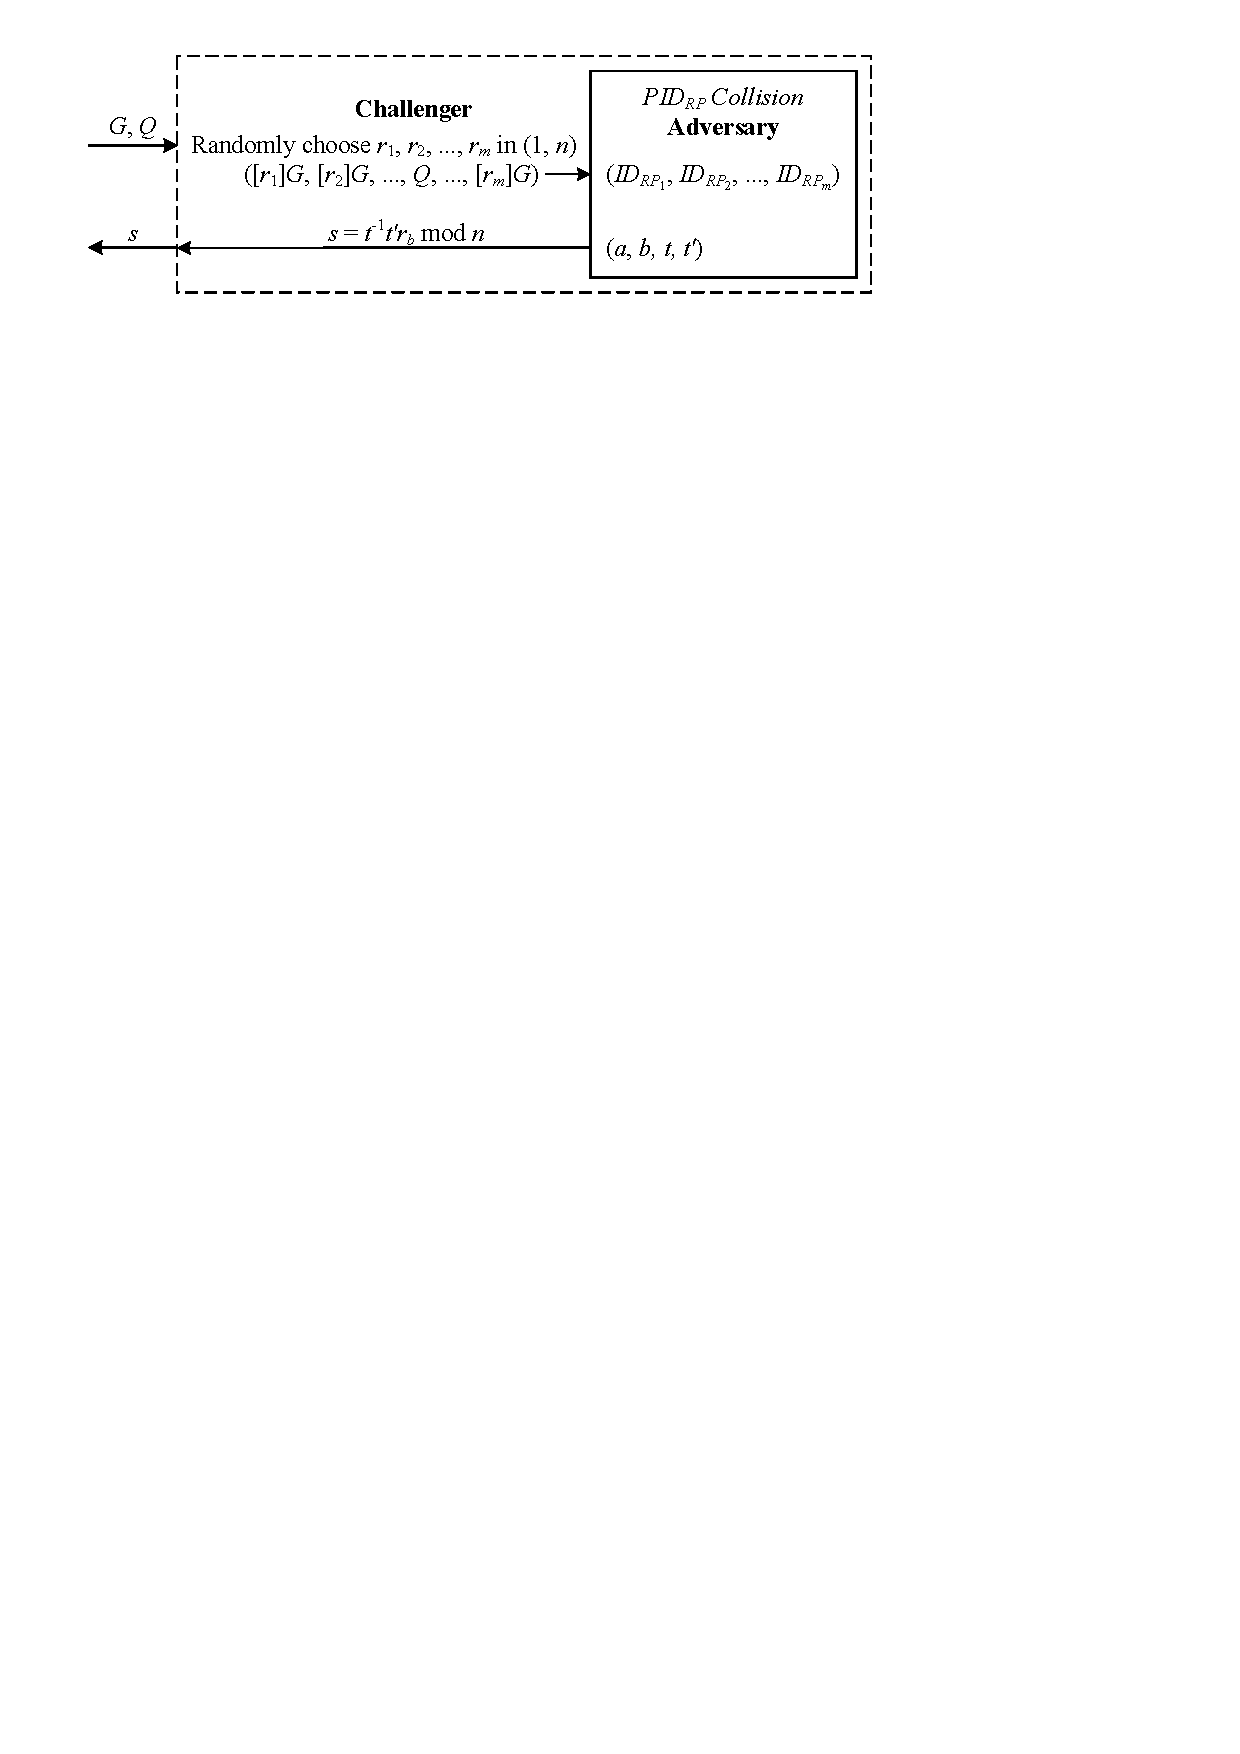
\includegraphics[width=0.97\linewidth]{fig/ecdlp_algorithm.pdf}
  \caption{The PPT algorithm $\mathcal{D}^*_c$ constructed based on the $PID_{RP}$ collision game, to solve the ECDLP problem.}
  \label{fig:ecdlp_algorithm}
\end{figure}

If the adversary succeeds in $\mathcal{G}_c$ and $[r_a]G$ happens to be replaced with $Q$,
  then $\mathcal{D}^*_c$ outputs $s=t^{-1}t'r_b =x$ because $[tr_a]G = [t]Q = [t'r_b]G$. For the adversary, $Q$ is indistinguishable from any other RP identities in the input set, as $[r_j]G$ is randomly replaced by the challenger.
Hence, the probability of solving the ECDLP using $\mathcal{D}^*_c$ is formulated as:
\begin{equation*}
{\rm Pr}\{\mathcal{D}^*_c(G, [x]G)=x\} = {\rm Pr}\{s = x\}={\rm Pr}\{a=j\}{\rm Pr}_s=\frac{1}{m}{\rm Pr}_s
\end{equation*}

%The probability of solving the ECDLP using $\mathcal{D}^*_c$ is denoted as ${\rm Pr}\{\mathcal{D}^*_c(G, [x]G)=x\}$.
%Due to the ECDLP assumption,
%    ${\rm Pr}\{\mathcal{D}^*_c(G, [x]G)=x\} = \epsilon_{c}(\lambda)$ becomes negligible when the security parameter $\lambda$ is sufficiently large.

If the probability of finding $t$ and $t'$ satisfying $[t]ID_{RP_j} = [t']ID_{RP_{j'}}$ is non-negligible,
    the adversary would have advantages  in $\mathcal{G}_c$ and ${\rm Pr}_s$ is non-negligible regardless of the security parameter $\lambda$.
Thus, we would find that ${\rm Pr}\{\mathcal{D}^*_c(G, [x]G)=x\}$ also becomes non-negligible  when $\lambda$ is sufficiently large, because $m$ is a finite integer and $m \ll 2^\lambda$.
\oldc
This violates the ECDLP assumption. Therefore, the probability of finding $t$ and $t'$ that satisfy $[t]ID_{RP_j} = [t']ID_{RP_{j'}}$ is negligible. \hfill $\square$


\newc
\vspace{2mm}
\noindent\textsc{\textbf{Theorem 2.} (User Identification of $TK$)} { $PID_U= [ID_U]PID_{RP}$ in $TK$ uniquely identifies an account at the RP designated by $PID_{RP}$, and this account is uniquely mapped to a user with $ID_U$.}

%In the identity token binding $PID_U$ and $PID_{RP}$, the user pseudo-identity $PID_U$ identifies the authenticated user with $ID_U$, % as $Acct = [ID_U][ID_{RP}]$,
%and only this user,  at the target RP with $ID_{RP} = [r]G$.}
%That is, in UPPRESSO, $Acct$ identifies the mapping $[ID_u][ID_{RP}]$.

\vspace{0.85mm}
\noindent\textsc{Proof.}
To issue an identity token requested for $PID_{RP}$, the honest IdP calculates $PID_U = [ID_U]PID_{RP}$ following Equation \ref{equ:PIDU} after authenticating the user with $ID_U$. The designated RP then calculates $Acct = [t^{-1}]PID_{U} = [ID_U]ID_{RP}$ following Equation \ref{equ:AccountNotChanged}.
$Acct = [ID_U]ID_{RP}$ is a \emph{permanent} identifier that is determined once the RP and the user have registered at the IdP. Therefore, $PID_U$ in $TK$ always identifies an $Acct$ at the designated RP, and $Acct$ is mapped to a user with $ID_U$.

Next, we prove that it \emph{uniquely} identifies one user in the system and one account at the RP. Since $\mathbb{E}$ is a finite cyclic group, $ID_{RP} = [r]G$ is also a generator on $\mathbb{E}$ of order $n$. Given a user with $ID_U$, $Acct = [ID_U]ID_{RP}$ is a unique point on $\mathbb{E}$ for any $u \in [1, n)$, which is uniquely associated to $ID_U=u$. \hfill $\square$

%According to the \dy~model, the RP may receive a $TK$ issued for another RP from a malicious RP script. However, if $PID_{RP} = [t]ID_{RP}$ holds, the RP can verify its designation by $PID_{RP}$ based on Theorem 1 and associates both $t$ and $TK$ with the current login.
%Then, the RP can calculate $Acct$ using $t$ and $PID_U$ following Eq.~\ref{equ:Account}. $Acct$ is determined only by $ID_U$ and $ID_{RP}$ based on Eq.~\ref{equ:AccountNotChanged}, which are permanent identifiers issued by the IdP during registration. Hence, $Acct$ cannot be manipulated by adversaries and is independent of logins. Therefore, in a user's multiple logins to the same RP, $PID_U$s are always mapped to one and only one $Acct$ at that RP.

%The detailed process of proof is shown in Appendix.

\newc
\vspace{2mm}
\noindent\textsc{\textbf{Theorem 3.} (Token Integrity)} { An identity token issued by the IdP cannot be forged or manipulated.}

%{\em Consider an arbitrary identity token $TK$ binding $PID_{RP}$ and $PID_U$. An honest RP accepts $TK$ if and only if $TK$ is valid, $PID_{RP}$ designates this RP with $ID_{RP}$, and $PID_U$ uniquely identifies a user account $Acct=[ID_U]ID_{RP}$ at this RP, indicating that $TK$ binds $ID_{RP}$ and $Acct$.}

%An honest RP accepts only identity tokens binding its pseudo-identity $PID_{RP}$ and the authenticated user's pseudo-identity $PID_U$, and actually binding $ID_{RP}$ and $Acct=[ID_U]ID_{RP}$, when $SK$ is held by only the IdP.

\vspace{0.85mm}
\noindent \textsc{Proof.} Identity tokens are generated and signed by the honest IdP using its private key, which is sufficiently protected at the IdP against adversaries.
%Meanwhile, the IdP's public key $PK$ is sent from the IdP to the RPs.
%and $PK$ which is pre-installed by an RP cannot be manipulated by adversaries.
With the pre-installed public key, an RP verifies the identity tokens it receives and rejects any forged or manipulated identity tokens. \hfill $\square$

%Due to the one-to-one mapping between (\emph{a}) the pair of $Acct$ and $PID_{RP}$ and (\emph{b}) the triple ($PID_U$, $PID_{RP}$, $t$), $TK$ binds $ID_{RP}$ and $Acct$ implicitly. \hfill $\square$

% A signed identity token binds $PID_{RP} = [t]ID_{RP}$ and $PID_U = [ID_U]PID_{RP}$, % $Acct$ and $ID_{RP}$ implicitly,
% and any breaking results in some failed checking or verification in the login flow as below.
%First of all, the identity token is signed by the honest IdP using $SK$ and verified by the RP using $PK$, so any modification will be rejected by the RP.
% According to the proof of RP designation, % there is no $t' \neq t$ but satisfying that $PID_{RP} = [t]ID_{RP_j} = [t']ID_{RP_{j'}}$.
% $PID_{RP}$ identifies only the RP with $ID_{RP}$; according to the proof of user identification, $PID_U$ identifies only the user with $Acct = [ID_U]ID_{RP}$ at the RP.
%Therefore, the identity token explicitly binding $PID_U$ and $PID_{RP}$, matches \emph{only} one $ID_{RP}$ and \emph{only} one $Acct = [t^{-1}]PID_{U}$.
%Therefore, $Acct$ and $ID_{RP}$ are actually bound in the token by the IdP's signatures,


\vspace{2mm}
\noindent{\textsc{\textbf{Theorem 4.} (Token Confidentiality)}} { An identity token is accessible only to its designated RP, besides the requesting user and the IdP.}
%An identity token is accessible to only the authenticated user and the target RP, in addition to the IdP signing this token.

\vspace{0.85mm}
\noindent\textsc{Proof.}
An identity token is generated by the IdP and then sent to the requesting user (i.e., its IdP script).
The IdP script verifies if $ID_{RP}$ specified in a verified RP certificate is designated by $PID_{RP}$ in the identity token and forward the token to the correct RP script, which is downloaded from the origin of $Enpt_{RP}$ specified also in the RP certificate. %Because the IdP script calculates $PID_{RP} =[t]ID_{RP}$ based on $ID_{RP}$ in this verified RP certificate, this RP is designated in the identity token and will receive the token from the RP script.
As all the communications between the IdP, RPs, and users are protected by HTTPS and two scripts communicate with each other through restricted \verb+postMessage+ HTML5 channels, according to the conclusions of the \dyu\ model, the identity tokens cannot be leaked to any other entities. \hfill $\square$


\vspace{2mm}
\noindent\textsc{\textbf{Theorem 5.} (Security)} {\usso\ is secure.}

\vspace{0.85mm}
\noindent\textsc{Proof.}
According to the formal analysis on SSO security \cite{SPRESSO, FettKS14},
    an SSO system satisfying the following two requirements is considered security in the first adversarial scenario: (\emph{a}) an adversary never obtains a valid identity token of an honest user and presents it to an honest RP, and (\emph{b}) an honest user never presents a valid identity token that is not issued for herself to an honest RP.
%(\emph{a}) an adversary never presents an identity token that is accepted by an honest RP to derive an honest user's account at this RP and (\emph{b}) an honest user never presents an identity token that is accepted by an honest RP to derive another user's account at this RP.


%In a secure SSO that is robust against impersonation attacks, an honest user should be able to prove her identity to the target RP with an identity token issued by the IdP. As pseudo-identities are used in \usso, an RP needs to verify that ({\em a}) $PID_{RP}$ in the received identity token is a transformation from its own $ID_{RP}$ and tied to the current login, which requires {\em RP designation}; and ({\em b}) $PID_U$ included in the identity token can be associated with a unique, long-term user account it maintains, which requires {\em user identification}. Besides, the identity token for an honest RP should not be intercepted by malicious users or RPs, requiring the {\em confidentiality of identity tokens}, nor be forged or tampered with to include a fake $PID_U$ or $PID_{RP}$, requiring the {\em integrity of identity tokens}.

Following the login flow of \usso, since the confidentiality and integrity of identity tokens are satisfied, no adversary could obtain a valid identity token that is issued to an honest user for accessing an honest RP. %and accepted by an honest RP.
Meanwhile, if an adversary presents an identity token to an honest RP, which may be issued to the adversary for accessing another RP or to an honest user for accessing a colluding RP, RP designation and user identification ensure that from this identity token, the honest RP does not derive an honest user's account.
%Meanwhile, $PID_U$ can only be calculated by the IdP and the user, since no one else knows or could intercept $u$ according to the DYU model. \oldc

According to the login flow and the \dyu\ model, an honest user always obtains identity tokens issued to herself, because $PID_U$ is calculated based on her own identity.
  %% which is protected against adversaries. 这一句,对于security没有用,protecting u是用于privacy。
The confidentiality and integrity of identity tokens ensure that an honest user never presents any token issued to someone else to an honest RP. Finally, with user identification,\footnote{\newc RP designation is a precondition of user identification in \usso, but this may not always be necessary for other SSO systems.} her identity tokens are always associated to her account at the target RP.
%According to the conclusions of the DYU model, $PID_U$ is calculated based on the user when the IdP issues an identity token for an authenticated user.
%Moreover, because the confidentiality and integrity of identity tokens are satisfied, an honest user never presents a valid token that is issued to other users.
%When the user identification is satisfied, this token always derives this honest user's account.
%So, an honest user never presents an identity token that is accepted by an honest RP to derive another user’s account at this RP.

Thus, \usso\ is a secure SSO system.
\hfill $\square$

%Finally, according to Theorems 1, 2, 3, 4, and 5, UPPRESSO is secure.

\subsection{Privacy}
\label{sec-:analysis}
\usso\ effectively prevents privacy threats introduced by IdP-based login tracing and RP-based identity linkage in the second and third adversarial scenarios, respectively.

\newc
First, we show that an honest-but-curious IdP cannot trace a user's login activities. In \usso, a user sends an identity-token request in each login to the IdP, %(Step 3.1 in Section~\ref{implementations})
which reveals only the target RP's \emph{ephemeral} pseudo-identity $PID_{RP}$ along with the user's identity $ID_U$.
The IdP cannot (\emph{a}) associate multiple logins with different $PID_{RP}$s to a given RP,
 or (\emph{b}) distinguish a login to one RP from other logins to another RP based on their $PID_{RP}$s,
 because to the IdP, $PID_{RP}$ is \emph{indistinguishable} from random variables. We prove this in Theorem 6.

\vspace{2mm}
\noindent{\textsc{\textbf{Theorem 6.} (Privacy against the IdP)}} { In \usso, the IdP cannot distinguish $PID_{RP} = [t]ID_{RP}$ from a random variable on $\mathbb{E}$, where $t$ is random in $\mathbb{Z}_n$.} %and unknown to the IdP.}

\vspace{0.85mm}
\noindent \textsc{Proof.}
Consider a finite cyclic group $\mathbb{E}$ where the number of points on $\mathbb{E}$ is $n$.
Because $G$ is a generator of order $n$, $ID_{RP} = [r]G$ is also a generator on $\mathbb{E}$ of order $n$. According to the \dyu\ model, $t$ is randomly chosen in $\mathbb{Z}_n$ and kept unknown to the IdP. Therefore, $PID_{RP} = [t]ID_{RP}$ is \emph{indistinguishable} from a point $Q$ that is randomly chosen on $\mathbb{E}$ \cite{oprf-proved,voprf-proved}.\footnote{\newc This property has been actually proved in OPRFs \cite{oprf-proved,voprf-proved}, where the OPRF server works similarly to the IdP and learns \emph{nothing} about a client's inputs or outputs of the evaluated pseudorandom function.} \hfill $\square$

%In order to receive $[k]Q$ for any given $Q$ on $\mathbb{E}$,
%    an OPRF client first generates a random number $e$, converts $Q$ to $[e]Q$,
%        and sends $[e]Q$ to the server.
%Then, the OPRF server returns $[ek]Q$, and the client obtains $[k]Q$ by using $e$.


%Consider a user's two arbitrary logins to an RP where $PID^{i}_{RP} = [t]ID_{RP}$ and $PID^{i'}_{RP} = [t']ID_{RP}$, and her another login to another RP where $PID^{i''}_{RP'} = [t'']ID_{RP'}$. According to the \dyu\ model, $t$, $t'$, and $t''$ are randomly selected by the IdP script and shared only with the corresponding RP through the RP script, so they are unknown to the IdP. As stated in Theorem 2, $ID_{RP} = [r]G = Q$ and $ID_{RP'} = [r']G = P$, where $P$ and $Q$ are two different points on the curve $\mathbb{E}$. Therefore, in the IdP's view, $[t]Q$, $[t']Q$, and $[t'']P$ are three random points on $\mathbb{E}$ when $t$, $t'$, and $t''$ are random and they are indistinguishable \cite{oprf-proved}. \hfill $\square$

%as well as from a $PID_{RP}$ generated in an arbitrary login for an arbitrary user to log in to an

%\textcolor{blue}{The information accessible to the IdP and derived from the RP's identity, is only $PID_{RP}$ in identity-token requests, where $PID_{RP} = [t]ID_{RP}$ is calculated by a user. % and $t$ is kept secret to the IdP.
%So the prevention against the IdP-based login tracing in UPPRESSO is expressed formally as below.}


\vspace{2mm}

In the third adversarial scenario, malicious RPs collude with malicious users.
First of all,
    in each login an RP with $ID_{RP}$ learns nothing about $ID_U$ from $Acct = [ID_U]ID_{RP}$, due to the ECDLP problem.
Thus,
given a shared view of the logins to the colluding RPs by malicious users,
    the adversaries attempt to link logins by an honest user but visiting different malicious RPs.
To show that \usso\ prevents such linkage, we prove in Theorem 7 that the adversaries cannot decide whether two logins visiting different malicious RPs are initiated by one honest user or not. %a login initiated by $U'$ to some of the $c$ malicious RPs
They cannot even associate a login visiting some malicious RP by an honest user with a subset of logins visiting another RP.

Let us investigate the knowledge that an RP obtains from each login. In \usso, an RP receives a random number $t$ and an identity token enclosing $PID_{RP}$ and $PID_U$ in each login. Meanwhile, it knows its own identity $ID_{RP}$ and derives the user's account $Acct$.
Because $PID_{RP}$ and $PID_U$ can be deduced from $ID_{RP}$ and $Acct$ with $t$, respectively, we ignore duplicated elements and define an RP's knowledge about a login as $L =(ID_{RP}, t, Acct)=(ID_{RP}, t, [ID_{U}]ID_{RP})$.


\vspace{2mm}
\noindent \textsc{\textbf{Theorem 7.} (Privacy against Colluding RPs)} { Given
    the logins visiting $c$ malicious RPs by $v$ colluding users, denoted as
 $\mathfrak{L}=\left \{ \begin{matrix}
L_{1,1},&L_{1,2},&\cdots,&L_{1,c}\\
L_{2,1},& L_{2,2},&\cdots,&L_{2,c}\\
\cdots,&\cdots,&L_{i,j},&\cdots\\
L_{v,1},&L_{v,2},&\cdots,&L_{v,c}
\end{matrix}\right\}$, where
 $L_{i, j}=([r_j]G, t_{i,j}, [u_ir_j]G)$ for $1 \le i \le v$ and $1 \le j \le c$,
the colluding adversaries cannot link a login visiting a malicious RP by some honest user
    to any subset of logins visiting another one,
  i.e., cannot decide whether $U'$ is in $\{{U''_1}, {U''_2}, \cdots, {U''_w}\}$ or randomly chosen from the universal user set,
    when a login visiting some malicious RP by a honest user $U'$ is denoted as $L'$,
     and the logins visiting another RP by some honest users $\{{U''_1}, {U''_2}, \cdots, {U''_w}\}$ are denoted as $\mathbb{L}'' = \{L''_k\}$ for $1 \leq k \leq w$,
     where $L' = ([r_{j'}]G, t', [u'r_{j'}]G)$, $L''_k = ([r_{j''}]G, t''_k, [u''_kr_{j''}]G)$, $u' \neq u_i$, $u''_k \neq u_i$,
     $j' \in [1,c]$, $j'' \in [1,c]$ and $j' \neq j''$.}

\vspace{0.85mm}
\noindent\textsc{Proof.}
We define an RP-based linkage game $\mathcal{G}_r$ between an adversary and a challenger,
    to describe this privacy threat:
 the adversary receives $\mathfrak{L}$, $L'$ and $\mathbb{L}''$ from the challenger,
 and outputs the result $s = 1$ if it decides $U'$ is in $\{{U''_1}, {U''_2}, \cdots, {U''_w}\}$
  or $s=0$ if $U'$ is randomly chosen from the universal user set.
Thus, the adversary succeeds in $\mathcal{G}_r$ with an advantage $\mathbf{Adv}_{A}$ as below:
\begin{align*}
&{\rm Pr}_1={\rm Pr}\{\mathcal{G}_r(\mathfrak{L}, L', \mathbb{L}'' | u' \in \{{u''_1}, {u''_2}, \cdots, {u''_w}\})=1\} \\
&{\rm Pr}_2={\rm Pr}\{\mathcal{G}_r(\mathfrak{L}, L', \mathbb{L}'' | u' \in \mathbb{Z}_n)=1\}\\
&{\mathbf{Adv}}_{A}=|{\rm Pr}_1-{\rm Pr}_2|
\end{align*}

As depicted in Figure \ref{fig:dalgorithm},
    we design a PPT algorithm $\mathcal{D}^*_r$ based on $\mathcal{G}_r$,
     to solve the elliptic curve decisional Diffie-Hellman (ECDDH) problem:
 given $(G, [x]G$, $[y]G$, $[z]G)$, decide whether $z$ equals to $xy$ or is randomly chosen in $\mathbb{Z}_n$,
    where $G$ is a point on an elliptic curve $\mathbb{E}$ of order $n$, and $x$ and $y$ are integers randomly and independently chosen in $\mathbb{Z}_n$.

%Therefore, according to the ECDDH assumption,
%    the advantage of using $\mathcal{D}^*_r$ to decide whether $z$ equals to $xy$ or not,
%    i.e., $\mathbf{Adv}^*_{A} = |{\rm Pr}^*_1 - {\rm Pr}^*_2| = \epsilon_{r}(\lambda)$, becomes negligible when the security parameter $\lambda$ is sufficiently large,
%        where
%\begin{align*}
%&{\rm Pr}^*_1 =  {\rm Pr}\{\mathcal{D}^*(G, [x]G, [y]G, [xy]G)=1\} \\
%&{\rm Pr}^*_2 =  {\rm Pr}\{\mathcal{D}^*(G, [x]G, [y]G, [z]G)=1\}
%\end{align*}
%
The algorithm $\mathcal{D}^*_r$ works as below.
Upon receiving an input $(G, Q_1=[x]G, Q_2=[y]G, Q_3=[z]G)$ of $\mathcal{D}^*_r$,
 the challenger chooses
 $\{u_1, u_2, \cdots, u_v\}$, $\{r_1, r_2, \cdots, r_c\}$, $\{t_{1, 1}, t_{1, 2}, \cdots, t_{v, c}\}$ randomly in $\mathbb{Z}_n$ for $1 \le i \le v$ and $1 \le j \le c$,
  where $[r_{j}]G \neq Q_2$ (i.e., $r_j \neq y$),
  to assign $L_{i, j}=([r_j]G, t_{i,j}, [u_ir_j]G)$.
Then,
 it randomly chooses $j' \in [1, c]$ and $t'$ in $\mathbb{Z}_n$, to assign $L' = ([r_{j'}]G, t', [r_{j'}]Q_1) = ([r_{j'}]G, t', [xr_{j'}]G)$.
% Here, $L'$ represents the knowledge of the login visiting $RP_{j'}$ by a user with $ID_U = x$.

Next, the challenger randomly chooses $j'' \in [1, c]$ but $j'' \neq j'$.
It replaces $L_{i, j''}$ with $(Q_2, t_{i,j''}, [u_i]Q_2) = ([y]G, t_{i,j''}, [u_iy]G)$ for $1 \leq i \leq v$;
that is, $ID_{RP_{j''}} = Q_2 = [y]G$ in $\mathfrak{L}$.
It also chooses $\{u''_1, u''_2, \cdots, u''_w\}$, $\{t''_1, t''_2, \cdots, t''_w\}$ randomly in $\mathbb{Z}_n$,
    where $[u''_k]G \neq Q_1$ (i.e., $u''_k \neq x$) and $u''_k \neq u_i$ for $1 \leq k \leq w$,
    to assign $L''_k = (Q_2, t''_k, [u''_k]Q_2) = ([y]G, t''_k, [u''_ky]G)$.
Finally,
the challenger randomly chooses $d \in [1, w]$, and replaces $L''_d$ with $(Q_2, t''_d, Q_3) = ([y]G, t''_d, [z]G)$.
Here, $\mathbb{L}'' = \{L''_{k; 1 \leq k \leq w}\}$ represents the knowledge of the logins
        visiting the $j''$-th RP %with $[y]G$
         by
    $w$ users with $\{u''_1, u''_2, \cdots, u''_{d-1}, z/y, u''_{d+1}, \cdots, u''_w\}$.
When the adversary receives $\mathfrak{L}$, $L'$, and $\mathbb{L}''$,
 it outputs $s$ which is further returned as the output of $\mathcal{D}^*_r$.

According to the above construction, % of $\mathfrak{L}$, $L'$ and $\mathbb{L}''$,
 $x$ is embedded as $ID_{U'}$ in $L'$ for $ID_{RP_{j'}} = [r_{j'}]G$,
 $z/y$ is embedded as $ID_{U''_d}$ in $\mathbb{L}''$ for $ID_{RP_{j''}} = [y]G$ together with $\{u''_1, u''_2, \cdots, u''_{d-1}, u''_{d+1}, \cdots, u''_w\}$, and $[r_{j'}]G$ and $[y]G$ are two RP identities in $\mathfrak{L}$.
Because $x$ is not in $\{u''_1, u''_2, \cdots, u''_{d-1}, u''_{d+1}, \cdots, u''_w\}$,
    the adversary succeeds with an output of $s=1$
     \emph{only if} $x = z/y$ holds.

The advantage $\mathbf{Adv}^*_{A}=|{\rm Pr}^*_1 - {\rm Pr}^*_2|$ of solving the ECDDH problem using $\mathcal{D}^*_r$ is deduced as below:
\begin{align*}
&{\rm Pr}^*_1 =  {\rm Pr}\{\mathcal{D}^*_r(G, [x]G, [y]G, [xy]G)=1\} \\
=&{\rm Pr}\{\mathcal{G}_r(\mathfrak{L}, L', \mathbb{L}'' | u' \in \{{u''_1}, {u''_2}, \cdots, {u''_w}\})=1\} = {\rm Pr}_1 \\
&{\rm Pr}^*_2= {\rm Pr}\{\mathcal{D}^*_r(G, [x]G, [y]G, [z]G)=1\} \\
=&{\rm Pr}\{\mathcal{G}_r(\mathfrak{L}, L', \mathbb{L}'' | u' \in \mathbb{Z}_n)=1\} = {\rm Pr}_2\\
&\mathbf{Adv}^*_{A}=|{\rm Pr}^*_1-{\rm Pr}^*_2|=|{\rm Pr}_1-{\rm Pr}_2|={\mathbf{Adv}}_{A}
\end{align*}

\begin{figure}[tb]
  \centering
  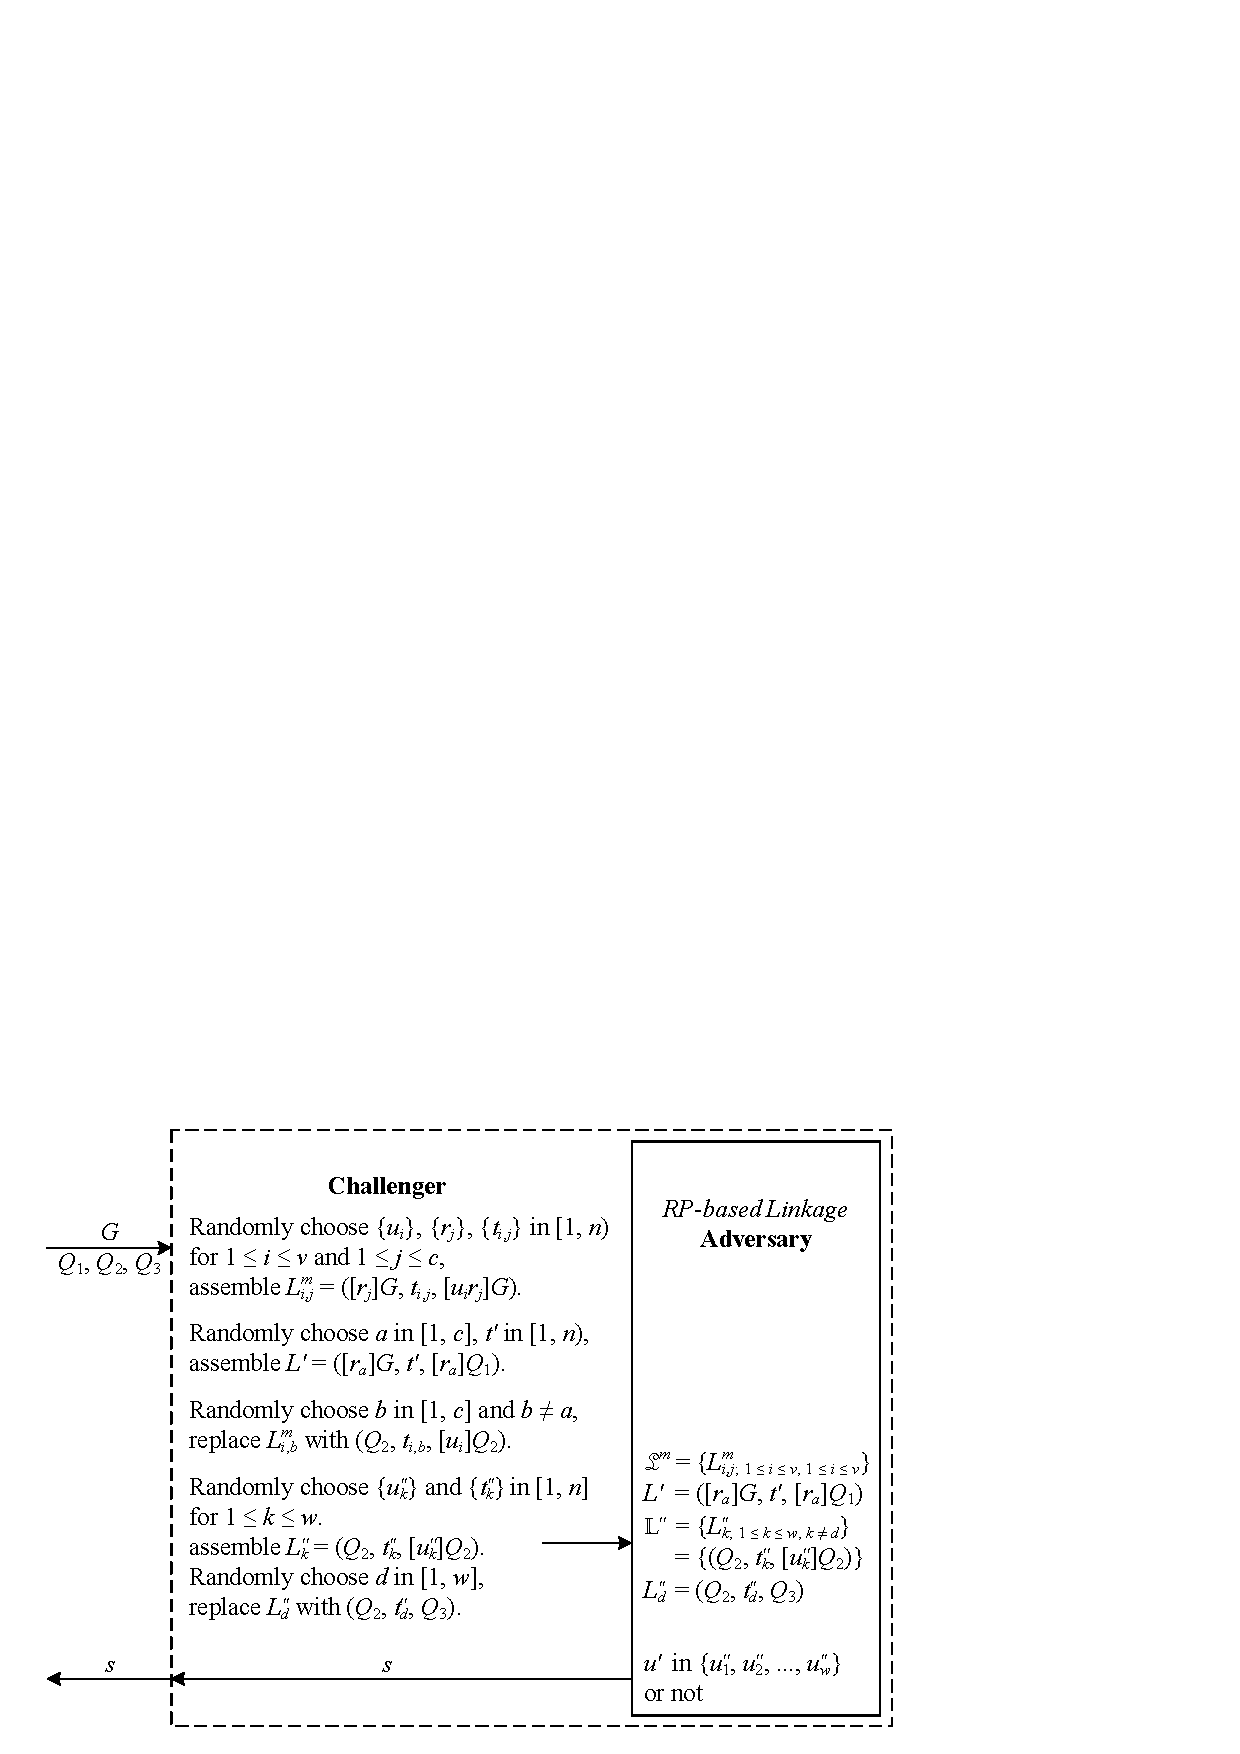
\includegraphics[width=1.0\linewidth]{fig/rp-linkage-game.pdf}
  \caption{The PPT algorithm $\mathcal{D}^*_r$ constructed based on the RP-based identity linkage game, to solve the ECDDH problem.}
  \label{fig:dalgorithm}
\end{figure}


If in $\mathcal{G}_r$ the adversary has non-negligible advantages,
    then $\mathbf{Adv}^*_{A}={\mathbf{Adv}}_{A}$ is also non-negligible regardless of the security parameter $\lambda$.
This violates the ECDDH assumption.
Therefore, the adversary has no advantages in $\mathcal{G}_r$ and cannot decide whether $L'$ is initiated by a user in \{${U''_1}, {U''_2}, \cdots, {U''_w}$\} or the universal user set.
\hfill $\square$

\oldc

